\documentclass[report]{subfiles}
\begin{document}
    \chapter{METHODOLOGY}
    \section{Flowchart}
    \begin{figure}[H]
        \centering
        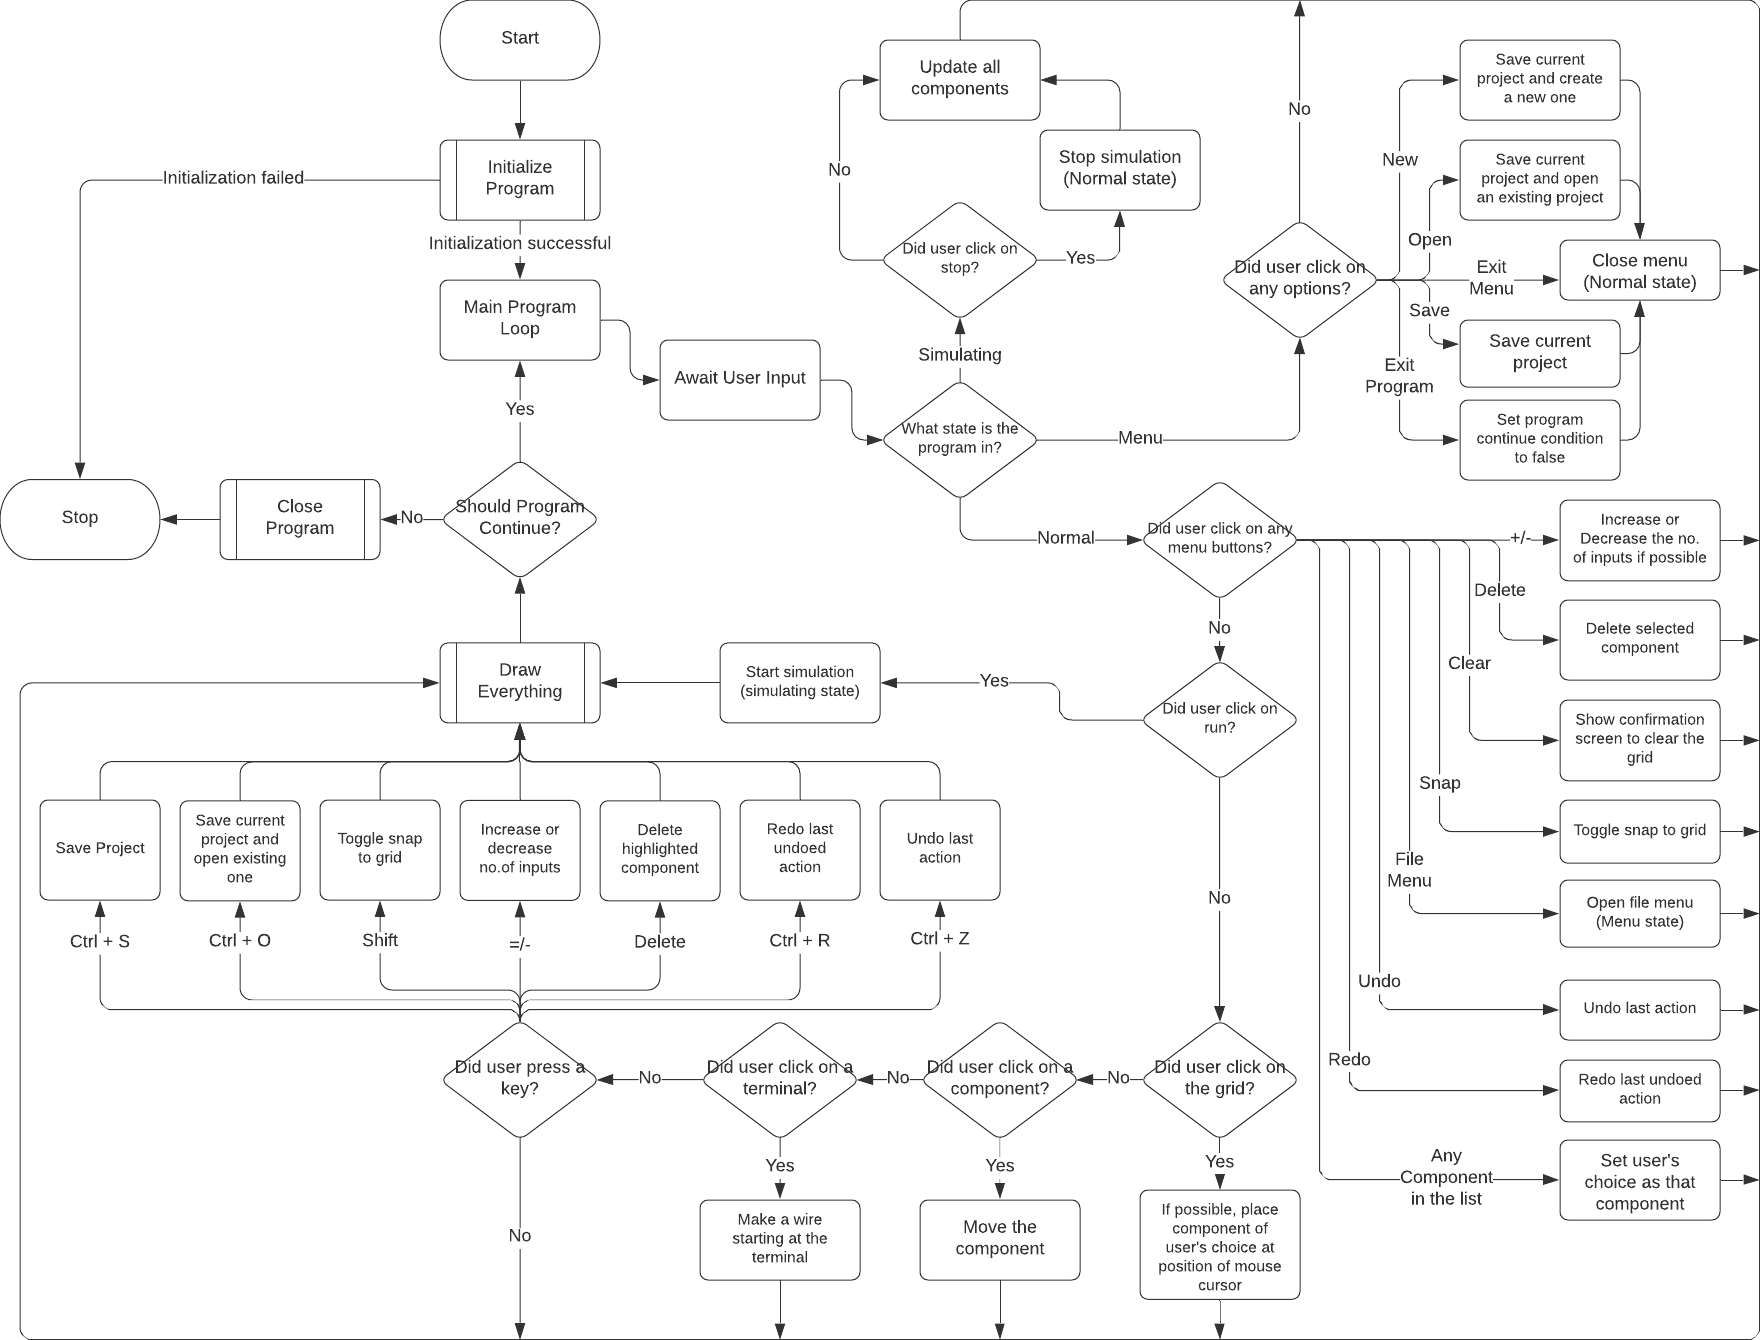
\includegraphics[width=\textwidth]{graphics/Flowchart.png}
        \caption{Flowchart of the program}
    \end{figure}
    \newpage
    \section{Working of the program}
    Working of the program can be described in the following three steps: 
    \subsection{Initialize}
    When the program is launched, initialization is carried out. If initialization is unsucessful, the program will display and error and quit. During this process, the libraries used by the program (SDL2 and SDL2\_ttf) are initialized. Then the SDL window and renderer are created. Fonts used to display text in the program are loaded and then a character map is created using the fonts. Since SDL2\_ttf ant the fonts are no longer required after the character map has been created, the fonts get closed and SDL2\_ttf is quit.\\
        \textbf{\texttt{Algorithm for Inititalizing}}
        \begin{verbatim}
initialize SDL
did SDL initialize successfully?
  yes: continue
  no : display error
     exit program
create SDL window
create SDL renderer
were the window and renderer created successfully?
  yes: continue
  no: display error
    exit program
initialize the grid
  fill grid with -1
initialize menu
  set dimensions and positions for all buttons
initialize SDL_ttf
did SDL_ttf initialize successfully?
  yes: continue
  no : display error
       exit program
load fonts
were fonts loaded successfully?
  yes: continue
  no : display error
       exit program
create character map
  create textures for all characters to be used
close fonts
close SDL_ttf
        \end{verbatim}
    \subsection{Loop}
    All user interaction, simulation and rendering happen inside the main program loop. During each iteration of the loop, the program waits for user input and then processes it as shown in the flowchart. Then all components of the program are rendered (drawn) onto the screen. If the simulation is running then all the components get updated. The loop continues to run until the user quits (presses the X button in title bar or presses Alt+F4) or exits program from the menu.\\
        \textbf{\texttt{Algorithm for Loop}}
        \begin{verbatim}
loop if program continue condition is true{
  await user input
  what state is program in?
    normal:
      if user clicked on RUN
        start simulation
      if user clicked on + or user pressed = key
        increase no. of inputs of current choice if possible
      if user clicked on - or user pressed - key
        decrease no. of inputs of current choice if possible
      if user clicked on Undo or user pressed Ctrl + z
        undo last action
      if user clicked on Redo or user pressed Ctrl + r
        redo last undoed action
      if user clicked on Delete Component or user pressed Delete key
        delete selected component on the grid
      if user clicked on Clear Grid
        show confirmation screen
          user clicked yes: empty the grid
      if user clicked on Snap to Grid or user held Shift
        toggle snapping to grid
        is snapping toggled on?
          yes: set snap button text to "Snap to Grid: On"
          no : set snap button text to "Snap to Grid: Off"
      if user clicked on File Menu
        open the menu
      if user clicked on any component in the list
        set user's choice to be that component
      if user pressed Ctrl + o
        save current project and open existing one
      if user pressed Ctrl + s
        save project
      if user clicked on component on the grid
        move the component
      if user clicked on terminal
        make wire starting at that terminal
      if user clicked on the grid
        if possible place user's choice of component on the grid
        at current mouse cursor position
    simulating:
      if user clicked on STOP
        stop simulation
      update all components
    menu:
      if user clicked on Save:
        save current project
        close menu
      if user clicked on New:
        save current project and create a new one
        close menu
      if user clicked on Open:
        save current project and open an existing one
        close menu
      if user clicked on Exit Menu:
        close menu
      if user clicked on Exit Program:
        set program continue condition to false 
        close menu
  draw everything
    draw menu
    draw grid
    draw components
    draw wires
}
        \end{verbatim}
    \subsection{Close}
    After the program exits from the loop, it calls some clean up function which destroy the textures, window and renderer and frees memory.\\
        \textbf{\texttt{Algorithm for Closing}}
        \begin{verbatim}
destroy all textures
destroy window
destroy renderer
quit SDL
exit program
        \end{verbatim}
\end{document}
